\documentclass[a4paper,10pt]{article}

\usepackage[spanish]{babel}
\usepackage[utf8]{inputenc}
\usepackage{geometry}
\usepackage{graphicx} % Required for inserting images
\geometry{margin=2.5cm}

\title{\textbf{Sistemas Operativos I}\\Informe de Trabajo Práctico Final}
\author{
Dallas Cañari Benites \\
Benjamín Alomar \\
Valentino Perticarari \\
Alan Hergenreder
}
\date{Junio 2026}

\begin{document}

\maketitle

\section{Roles y contribuciones}

En este trabajo práctico, cada integrante del equipo asumió un rol principal, manteniendo colaboración en la integración general del sistema.

\begin{itemize}
    \item \textbf{Dallas Cañari Benites - Ingeniero de comunicaciones (C)}

    \item \textbf{Alan Hergenreder - Gestor de recursos (C)}

    \item \textbf{Valentino Perticarati - Planificador y lógica anti-deadlock (Erlang)}

    \item \textbf{Benjamín Alomar - Integración, testing y documentación}
\end{itemize}

\section{Diseño}

\subsection{Arquitectura general}

El sistema implementado sigue una arquitectura distribuida compuesta por dos componentes principales: un \textit{Resource Manager Agent} desarrollado en C y un \textit{Job Scheduler} desarrollado en Erlang.

Cada nodo del sistema ejecuta ambas aplicaciones de forma independiente. El agente en C es responsable de la comunicación con otros nodos, el mantenimiento de los recursos locales y el descubrimiento dinámico de agentes en la red. Por otro lado, el scheduler en Erlang es responsable de generar trabajos, solicitar recursos y coordinar la ejecución de los jobs.

La comunicación entre ambos componentes se realiza mediante TCP utilizando la interfaz local definida en la consigna. A su vez, los agentes en C se comunican entre sí utilizando TCP para la reserva de recursos y UDP broadcast para el descubrimiento automático de nodos.

\subsection{Modelo de ejecución}

El sistema fue diseñado siguiendo un modelo concurrente que aprovecha las características de ambos lenguajes utilizados.

En el \textbf{agente desarrollado en C} se emplea un modelo orientado a eventos basado en \texttt{epoll}, combinado con un esquema multithreading de una cantidad fija de hilos. Todos esos hilos monitorean, mediante llamados a \texttt{epoll\_wait} sobre una misma instancia de \texttt{epoll} compartida, la totalidad de los descriptores activos del sistema. Esto incluye conexiones provenientes de otros agentes, conexiones del scheduler local, el socket UDP utilizado para el descubrimiento de nodos y los temporizadores asociados a tareas periódicas. Cuando alguno de estos descriptores genera un evento, únicamente uno de los hilos bloqueados en \texttt{epoll\_wait} es despertado para atenderlo. 

El \textbf{scheduler desarrollado en Erlang} utiliza el modelo de actores propio del lenguaje. Existe un proceso planificador central encargado de recibir los jobs, construir las peticiones correspondientes y crear un proceso independiente (\textit{handler}) para cada trabajo. Cada handler gestiona el ciclo de vida completo del job de forma concurrente. Además, un proceso supervisor monitorea exclusivamente al scheduler principal y lo reinicia automáticamente si finaliza de manera inesperada.

Esta combinación permite aprovechar la eficiencia de C para el manejo de eventos de red y la facilidad de Erlang para desarrollar sistemas concurrentes y tolerantes a fallos.

\subsection{Componente agente C}

El agente C actúa simultáneamente como servidor y cliente dentro del sistema distribuido.

Como servidor, acepta tanto las conexiones entrantes de otros agentes remotos como la conexión local del scheduler Erlang, y atiende las solicitudes que le llegan por cada una: a los agentes les procesa los mensajes \texttt{RESERVE} y \texttt{RELEASE} sobre sus recursos locales, y al scheduler le atiende los comandos \texttt{JOB\_REQUEST}, \texttt{JOB\_RELEASE} y \texttt{GET\_NODES}.

Como cliente, establece conexiones TCP hacia otros agentes (si todavia no se hizo) cuando necesita solicitar recursos
remotos para un determinado job, y les envia los mensajes \texttt{RESERVE} y \texttt{RELEASE} correspondientes.

Internamente, el agente mantiene las siguientes estructuras:
\begin{itemize}
    \item \texttt{fd\_table}: descriptores de archivo agregados a la instancia de \texttt{epoll}.
    \item \texttt{local\_resources}: recursos locales disponibles.
    \item \texttt{agent\_table}: nodos descubiertos en la red.
    \item \texttt{job\_table}: jobs activos recibidos del scheduler.
    \item \texttt{reservation\_table}: reservas concedidas o encoladas correspondientes a solicitudes recibidas por una conexión de agente, incluyendo el caso particular en que el propio nodo se solicita recursos a sí mismo a través de una conexión consigo mismo, comportándose como un agente más.
\end{itemize}

\subsection{Componente scheduler Erlang}

El scheduler implementado en Erlang es el encargado de coordinar la ejecución de los trabajos y de interactuar con el agente local desarrollado en C.

Durante la inicialización establece una conexión TCP con el agente, solicita de forma síncrona el mapa de nodos disponibles mediante el comando \texttt{GET\_NODES} y almacena esa información en una tabla ETS que mantiene el estado de los recursos disponibles en cada nodo.

El sistema puede funcionar en dos modos:

\begin{itemize}
    \item \textbf{Modo random}: genera automáticamente una cantidad configurable de jobs con requerimientos aleatorios de CPU, MEMORIA y GPU.
    \item \textbf{Modo manual}: permite que el usuario ingrese manualmente los pedidos desde la consola.
\end{itemize}

Cada job recibe un identificador único generado mediante \texttt{erlang:unique\_integer()}.

El scheduler analiza cada pedido, determina cómo distribuir los recursos entre los distintos nodos disponibles y construye los mensajes \texttt{JOB\_REQUEST} correspondientes.

Para cada trabajo se crea un proceso independiente (\textit{handler}) encargado de:

\begin{itemize}
    \item registrar el job en la tabla ETS de pendientes,
    \item enviar el \texttt{JOB\_REQUEST} al agente local,
    \item esperar la respuesta del agente,
    \item manejar los casos \texttt{JOB\_GRANTED}, \texttt{JOB\_DENIED} o timeout,
    \item devolver automáticamente los recursos reservados una vez resuelto el
    resultado del job, ya sea que este haya sido concedido, rechazado o haya
    vencido por timeout,
    \item enviar el correspondiente \texttt{JOB\_RELEASE} cuando el trabajo finaliza,
    \item registrar el resultado en el archivo de logs,
    \item informar al scheduler la finalización del job.
\end{itemize}

Las respuestas provenientes del agente son recibidas por el proceso (\texttt{tcp\_deliver}), que actúa como despachador: recibe todos los mensajes TCP, identifica el \texttt{JobID} correspondiente y reenvía cada respuesta al proceso handler encargado de ese trabajo utilizando la tabla ETS de pendientes.
\subsection{Decisiones de diseño}

Durante el desarrollo del sistema se tomaron diversas decisiones de diseño orientadas a mejorar la escalabilidad, la modularidad y la tolerancia a fallos.

\subsubsection{Decisiones de diseño en el agente C}

\paragraph{Uso de epoll para el manejo de conexiones}

Se utiliza una única instancia de \texttt{epoll}, monitoreada concurrentemente por un pool fijo de
hilos que llaman a \texttt{epoll\_wait} sobre ella. De esta forma se puede atender una gran cantidad
de conexiones TCP y UDP simultáneas con una cantidad acotada de hilos, aprovechando varios núcleos
del procesador. Además, todos los descriptores se agregan en modo \texttt{EPOLLET}
(\textit{edge-triggered}): como varios hilos comparten la misma instancia, esto asegura que ante
un evento solo uno de ellos sea despertado, y evita que ese mismo evento se vuelva a reportar
mientras no haya actividad nueva sobre el descriptor, siempre que el hilo que lo atiende lea o
escriba hasta agotar los datos disponibles (hasta \texttt{EAGAIN}).

Mediante dicha instancia se monitorean:
\begin{itemize}
    \item las conexiones con otros agentes,
    \item la conexión con el scheduler local,
    \item los sockets de escucha, tanto para nuevas conexiones de otros agentes como para la conexión con el scheduler,
    \item el socket UDP de descubrimiento,
    \item temporizadores asociados al sistema.
\end{itemize}

Como distintos hilos pueden llegar a manejar eventos sucesivos sobre una misma conexión (por
ejemplo, una lectura y una escritura casi simultáneas), la lectura y la escritura de cada una se
protegen con mutex independientes, evitando que dos hilos operen a la vez sobre el mismo buffer.
De la misma manera, el cierre de una conexión se coordina mediante campos de estado propios de
cada entrada (un contador de referencias y una marca de cierre pendiente) junto con la tabla de
descriptores (\texttt{fd\_table}): mientras un hilo todavía está usando la conexión se evita que
otro la cierre por debajo, y el cierre efectivo (sacarla de \texttt{epoll}, cerrar el \texttt{fd}
y liberar su información asociada) se pospone hasta que ningún hilo la esté utilizando.

\paragraph{Establecimiento de una conexión}

Toda conexión TCP nueva, ya sea aceptada desde un socket de escucha o iniciada activamente hacia
otro agente, se incorpora al sistema siguiendo los mismos tres pasos: primero se acepta la
conexión entrante o se intenta establecer la saliente; luego se la agrega a la \texttt{fd\_table},
que crea su identificador (\texttt{id}) y la información asociada (\texttt{info}); y finalmente se
agrega el descriptor a la instancia de \texttt{epoll} para que sus eventos comiencen a ser
monitoreados.

\paragraph{Manejo de una desconexión}

Una conexión puede darse por finalizada por distintos motivos: una lectura que devuelve 0 bytes
(el otro extremo cerró), un error al leer o escribir sobre el socket, un evento
\texttt{EPOLLHUP}/\texttt{EPOLLERR} reportado por \texttt{epoll}, o el vencimiento del temporizador
asociado a un nodo. Según el caso, el agente sigue una secuencia distinta de pasos:

\begin{itemize}
    \item \textbf{Nodo caído por vencimiento de su temporizador}: se elimina la entrada
    correspondiente de \texttt{agent\_table}, buscándola por IP y puerto (los datos que guarda el
    propio temporizador), y se cierra y elimina de \texttt{fd\_table} el descriptor del
    temporizador.
    \item \textbf{Conexión con un agente perdida por cualquiera de los otros motivos}: se limpia
    el identificador de conexión guardado en la entrada de \texttt{agent\_table} correspondiente,
    sin eliminar la entrada en sí (el nodo puede seguir vivo y anunciándose); se liberan los
    recursos locales concedidos o encolados asociados a esa conexión; y se elimina la conexión de
    \texttt{fd\_table} y de \texttt{epoll}, cerrando el \texttt{fd}.
    \item \textbf{Conexión con el scheduler perdida}: se recorren todos los jobs activos de
    \texttt{job\_table}, enviando \texttt{RELEASE} a cada agente involucrado en cada uno para
    liberar los recursos que tuviera reservados o encolados; luego se elimina la conexión de
    \texttt{fd\_table} y de \texttt{epoll}, cerrando el \texttt{fd}, y se reinicia el identificador
    de conexión del scheduler.
\end{itemize}

\paragraph{Uso de temporizadores mediante timerfd}

Se utilizaron temporizadores integrados mediante \texttt{timerfd}, los cuales pueden ser 
gestionados por \texttt{epoll} como cualquier otro descriptor de archivo.

Esto permitió implementar tareas periódicas dentro del mismo ciclo de eventos sin necesidad 
de hilos adicionales, particularmente para:
\begin{itemize}
    \item envío periódico de mensajes \texttt{ANNOUNCE},
    \item detección de nodos inactivos.
\end{itemize}

\paragraph{Manejo de recursos}

\begin{itemize}
    \item \texttt{fd\_table}: tabla hash cuya clave es el descriptor de archivo (\texttt{fd}),
    protegida por un mutex para leer y agregar, además de un mutex para cada entrada. Guarda el tipo y la información de cada conexión o temporizador
    agregado a \texttt{epoll} (buffers, estado de cierre). Es necesaria para que cualquier hilo
    pueda recuperar el estado asociado a un evento de \texttt{epoll} y coordinar el cierre de una
    conexión entre varios hilos.
    \item \texttt{local\_resources}: un arreglo con un elemento por cada
    tipo de recurso local, cada uno con su propio mutex y su cola FIFO de solicitudes pendientes.
    Permite manejar los recursos propios.
    \item \texttt{agent\_table}: tabla hash cuya clave es \texttt{ip:puerto}, protegida por un único
    mutex. Guarda los nodos descubiertos en la red, sus recursos anunciados y, si existe, el
    identificador de la conexión establecida con cada uno. Permite decidir a qué nodos se les puede
    enviar una solicitud y reutilizar una conexión ya abierta en lugar de crear una nueva.
    \item \texttt{job\_table}: tabla hash cuya clave es \texttt{job\_id}, protegida por un único
    mutex. Guarda los jobs activos recibidos del scheduler junto con los pedidos que los componen.
    Es necesaria para poder liberar todos los recursos de un job (ante un \texttt{JOB\_RELEASE} o
    ante la caída del scheduler) y para saber cuándo un job tiene todos sus recursos concedidos.
    \item \texttt{reservation\_table}: tabla hash cuya clave es la tupla
    (\texttt{job\_id}, \texttt{src\_id}, \texttt{nombre\_recurso}), protegida por un único mutex.
    Guarda el estado (concedida o encolada) de cada reserva de un recurso local. Esa clave compuesta
    es necesaria porque un mismo \texttt{job\_id} puede pedir varios recursos distintos, y porque
    ese mismo \texttt{job\_id} puede repetirse entre distintas conexiones entrantes
    (\texttt{src\_id}); es lo que permite, ante un \texttt{RELEASE} o ante la caída de una
    conexión, encontrar exactamente qué reserva liberar sin confundirla con la de otro pedido.
\end{itemize}

Mantener estas responsabilidades en estructuras separadas permite actuar ante los distintos comandos evitando mezclar información con propósitos distintos.
\subsubsection{Decisiones de diseño en el scheduler Erlang}

\paragraph{Uso del modelo de actores}

Se eligió aprovechar el modelo de actores de Erlang para representar la concurrencia del sistema.

Cada job se ejecuta mediante un proceso independiente, lo que permite que múltiples trabajos avancen simultáneamente sin necesidad de mecanismos explícitos de sincronización compartida.

Además, el aislamiento entre procesos reduce el impacto de errores individuales.
Los procesos se comunican mediante paso de mensajes para coordinar su ejecución, mientras que el estado compartido necesario se mantiene en tablas ETS, que permiten acceso concurrente mediante operaciones atómicas.
\paragraph{Scheduler central y handlers independientes}

Delegar la gestión completa de cada job a un proceso handler independiente
(en lugar de manejarlo en el proceso scheduler principal) evita que un
trabajo lento o bloqueado impida procesar nuevos pedidos, y mantiene al
scheduler central liviano y enfocado únicamente en recibir jobs y despachar
handlers.

\paragraph{Despachador de respuestas TCP}

Se centralizó la lectura del socket en un único proceso (\texttt{tcp\_deliver}) en
lugar de que cada handler leyera directamente de la conexión compartida con el
agente C. Esto evita que múltiples procesos intenten leer simultáneamente del mismo
socket, y mantiene la comunicación TCP completamente desacoplada de la lógica
propia de cada trabajo.

\paragraph{Supervisión automática}

Se implementó un supervisor dedicado al proceso scheduler utilizando enlaces (\texttt{spawn\_link}) y captura de señales de salida (\texttt{trap\_exit}).

Si el scheduler termina por un error, el supervisor crea automáticamente una nueva instancia del proceso, actualiza su registro global y continúa monitoreándolo sin necesidad de reinicializar el resto del sistema.

En cambio, si el scheduler finaliza normalmente, el supervisor también termina su ejecución.

\paragraph{Uso de ETS para estado compartido}

Se utilizan dos tablas ETS con responsabilidades bien diferenciadas.

\noindent La tabla \texttt{pendientes} almacena, para cada job activo, su identificador,
el proceso handler encargado de gestionarlo y los descuentos de recursos
aplicados sobre los nodos. Esta información permite redirigir correctamente
las respuestas provenientes del agente y restaurar los recursos reservados
cuando un job finaliza, es rechazado o vence su timeout.

\noindent La tabla \texttt{recursos\_nodos} mantiene la disponibilidad de CPU, MEMORIA
y GPU de cada nodo, con una entrada independiente por cada combinación
\texttt{\{Nodo, TipoRecurso\} => Cantidad}, además de una entrada con el
orden de recorrido de los nodos utilizado al repartir un pedido entre varios.
Esto permite modificar las cantidades mediante \texttt{ets:update\_counter},
una operación atómica que evita condiciones de carrera cuando múltiples jobs
solicitan recursos simultáneamente. El mapa recibido inicialmente del agente
C (\texttt{maps:from\_list}) se usa únicamente como paso intermedio de
parseo antes de volcarse a esta tabla.

\noindent Al tratarse de tablas ETS públicas, todos los procesos del scheduler pueden
acceder concurrentemente a ellas sin necesidad de intercambiar mensajes
adicionales.

\paragraph{Distribución automática de recursos}

Cuando un job solicita una cantidad de recursos superior a la disponible en un único nodo, el scheduler intenta repartir dicha solicitud entre varios nodos disponibles.

\noindent Por ejemplo, si un job necesita cuatro CPUs y ningún nodo posee las cuatro disponibles, el scheduler puede construir una petición que combine recursos provenientes de distintos nodos.

\noindent Esta estrategia busca aprovechar mejor los recursos globales del sistema y aumentar la probabilidad de ejecución de los trabajos.

\noindent Durante este proceso, el scheduler realiza reservas locales descontando inmediatamente los recursos seleccionados de la tabla ETS mediante operaciones atómicas, antes de enviar el \texttt{JOB\_REQUEST}. De esta manera, otros jobs consideran esos recursos como ocupados y no pueden asignarlos simultáneamente. Si el trabajo finaliza correctamente (\texttt{JOB\_GRANTED}), es rechazado (\texttt{JOB\_DENIED}) o expira por timeout, dichas reservas se revierten automáticamente, restaurando los recursos en la tabla ETS y manteniendo consistente el estado local del scheduler.

\section{Problemas encontrados y soluciones}

\noindent Durante el desarrollo del agente en C surgieron varios problemas de concurrencia que se fueron detectando y corrigiendo a medida que se probaba el sistema. A continuación se describen los más relevantes.

\paragraph{Envío cruzado sobre un mismo fd}

Inicialmente cada fd se agregaba a \texttt{epoll} con la flag \texttt{EPOLLONESHOT}, buscando garantizar que un único hilo manejara ese descriptor a la vez. Esa garantía no cubría todos los casos: si llegaba un evento sobre la conexión de un agente, el hilo que lo recibía procesaba ese fd con normalidad, pero si en simultáneo llegaba un evento del scheduler que resultaba en mandarle un \texttt{RESERVE} a ese mismo agente (como parte de procesar un \texttt{JOB\_REQUEST}), un segundo hilo terminaba escribiendo sobre el mismo fd al mismo tiempo: \texttt{EPOLLONESHOT} solo evita que el propio evento de ese descriptor se entregue dos veces, pero no evita que otro camino de código, disparado por un evento distinto, acceda a él. La solución fue reemplazar ese mecanismo de sincronización por mutex (\texttt{mutex\_in} y \texttt{mutex\_out} en cada conexión), que protegen directamente la lectura y la escritura de cada una sin importar qué evento haya disparado el acceso.

\paragraph{Eventos entregados a conexiones ya cerradas}

Originalmente el dato que se guardaba junto a un fd en \texttt{epoll} era directamente la información de esa conexión. Al cerrar y eliminar un fd, si el sistema operativo reutilizaba ese mismo número de descriptor para una conexión nueva, un hilo podía llegar a procesar un evento que en realidad correspondía a la conexión vieja ya cerrada, operando por error sobre la conexión nueva que ahora ocupa ese mismo número de fd. La solución fue introducir la \texttt{fd\_table}: cada entrada guarda, además de la información de la conexión, un contador \texttt{reuse} que se incrementa cada vez que ese fd se reutiliza. El identificador que se le entrega a \texttt{epoll} (y que se guarda en otras estructuras como \texttt{agent\_table}) no es el fd solo, sino un valor de 64 bits que combina el fd con el valor de \texttt{reuse} vigente al momento de agregarlo. Así, cuando llega un evento, la función que recupera la conexión a partir de ese identificador puede comparar el \texttt{reuse} recibido contra el actual de la entrada: si no coinciden, el evento se descarta por corresponder a una conexión que ya no existe, en vez de operar por error sobre la conexión nueva que casualmente reutiliza el mismo fd.

\paragraph{Condición de carrera al registrar un job}

Al procesar un \texttt{JOB\_REQUEST}, inicialmente se enviaba el \texttt{RESERVE} correspondiente a cada recurso pedido a medida que se lo iba parseando de la solicitud, y recién al final se agregaba el job completo a la \texttt{job\_table}. Esto abría una ventana de carrera: si un agente respondía muy rápido con un \texttt{GRANTED} para el primer recurso pedido, esa respuesta podía procesarse antes de que el job existiera en \texttt{job\_table}, perdiéndose esa concesión o dejando inconsistente el conteo de recursos otorgados. La solución fue separar ambas etapas: primero se parsean todos los pedidos de la solicitud sin enviar nada, luego se agrega el job completo a \texttt{job\_table}, y solo después se procesa cada pedido enviando su \texttt{RESERVE} correspondiente, garantizando que el job ya esté registrado antes de que pueda llegar cualquier respuesta sobre él.

\paragraph{Mecanismo de descubrimiento de nodos}

Dejar de estar conectado con un agente no debe interpretarse como que ese nodo está caído, ya que puede tratarse solo de un problema de la conexión y no del nodo en sí. Se corrigió el manejo de la desconexión de un agente para que únicamente limpie el identificador de conexión de su entrada en \texttt{agent\_table}, sin eliminarla ni tocar su temporizador de anuncios, dejando que sea exclusivamente el vencimiento de ese temporizador el que determine si un nodo se considera caído. Además, se detectó que al actualizar los recursos de un nodo ya conocido no se actualizaba también la cantidad de recursos de la entrada, quedando desincronizada de la cantidad de valores efectivamente copiados si esa cantidad cambiaba entre un anuncio y otro. Se corrigió para que ambos datos se actualicen siempre juntos.

\section{Estrategia contra deadlock}

% Esto claramente se puede escribir mucho mas corto
\begin{itemize}
\item \textbf{Manejo de esperas prolongadas, supervisión y liberación controlada de
recursos}. Se implementó un mecanismo de recuperación ante situaciones en las que un job permanece esperando recursos durante un tiempo excesivo. La detección de estas situaciones se realiza desde el scheduler implementado en Erlang, donde cada job es ejecutado por un proceso independiente que monitorea el tiempo transcurrido mientras espera una respuesta del agente C, utilizando un timeout configurable.

Si dicho tiempo expira antes de recibir una respuesta satisfactoria, el sistema interpreta la situación como un posible deadlock o una condición de espera anormalmente larga. En ese caso, el proceso encargado del job registra el evento en el archivo de logs, envía un comando \texttt{JOB\_RELEASE} al agente C para liberar cualquier recurso que hubiese sido concedido parcialmente y restaura en la tabla ETS del scheduler los recursos que habían sido reservados localmente al construir la solicitud. De esta manera, tanto el agente C como el estado local del scheduler recuperan los recursos reservados, evitando inconsistencias y permitiendo que nuevos jobs puedan reutilizarlos

Esta estrategia unifica la supervisión de estados de espera prolongada con la liberación controlada de recursos, permitiendo detectar situaciones de posible interbloqueo, liberar recursos retenidos y garantizar el progreso del sistema. De este modo se reduce la probabilidad de deadlocks distribuidos y se evita la acumulación de recursos asignados a trabajos que no pueden completarse.
\end{itemize}

\section{Diagramas}

% Poner diagrama 1
 
% Poner diagrama 2

\begin{figure}[ht]
    \centering
    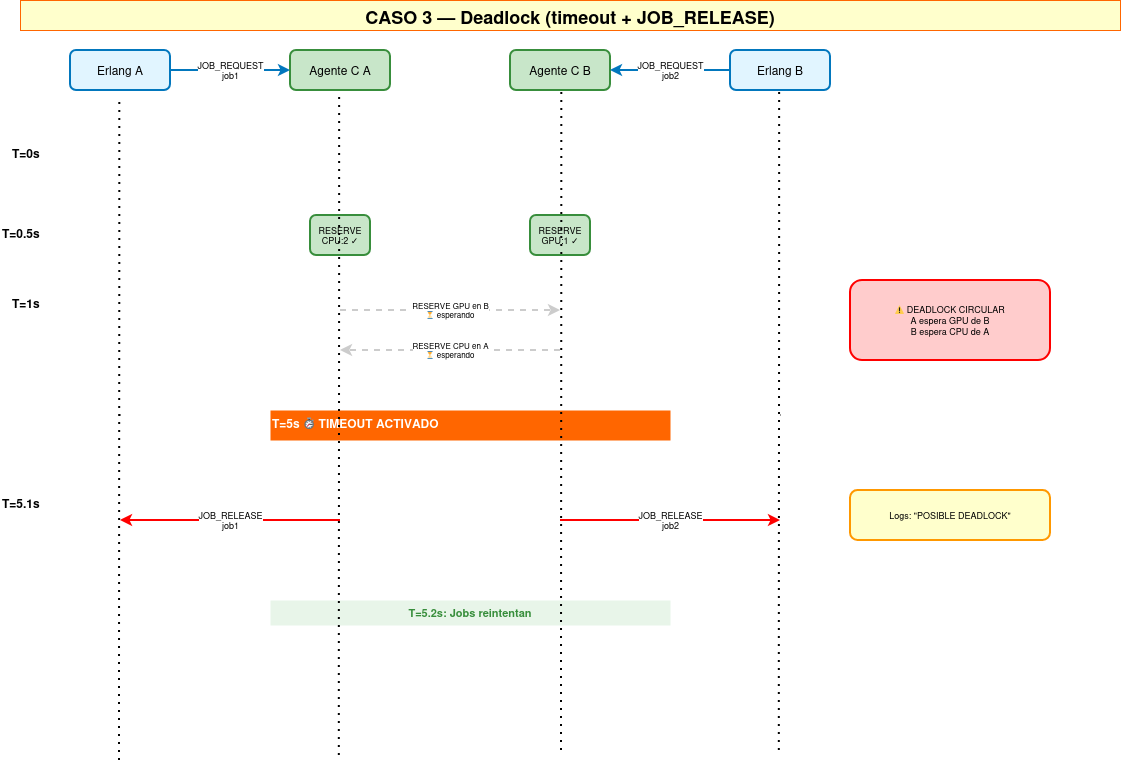
\includegraphics[width=1.1\linewidth]{caso3_deadlock.drawio.png}
    \label{fig:deadlock}
\end{figure}


\end{document}
